

\newpage
\subsection{Randomized algorithms}

\begin{enumerate}
  \item hello.

  \item motivation: improve runtimes for certain types of problems.

  \item Las Vegas: an algorithm which makes random choices during execution;
    which always produces the correct result \emph{or} correctly signals its
    failure, but whose runtime is probabilistic. If for a certain problem
    finding a solution is complex, but verifying a solution is easy, Las Vegas
    algorithms can be advantageous. A good example are NP-complete problems!

  \item Monte Carlo: an algorithm which makes random choices during execution;
    whose runtime is deterministic for any input, but one whose result is
    probabilistic (albeit usually correct with a high probability). As such they
    are comparable to approximation algorithms using randomness, but with Monte
    Carlo algorithms we are typically concerned with success/failure rather than
    a ratio of correctness.

  \item as an example of a Monte Carlo algorithm, I have chosen randomized
    quicksort (RandQS).

  \item first, let's briefly discuss regular quicksort. As you know, quicksort
    is a comparison-based sorting algorithm with average case $O(n \lg n)$ and
    worst case $O(n^2)$ number of comparisons:

    \begin{textred}
      \begin{alignat}{3}
        &\underline{\text{QS}}&&\\
        \quad&\text{average case:}&&\quad O(n \lg n),\\
                       &\text{worst case:}  &&\quad O(n^2).
      \end{alignat}
    \end{textred}

    The worst case occurs when using left-pivots on a sorted array; using
    right-pivots on a reversely sorted array; or when all of the list elements
    are the same, since in these cases, we split a length $n$ list into two
    subarrays of length $0$ and $(n - 1)$.

  \item randomized quicksort differs from regular quicksort only in the choice
    of pivot. Instead of choosing eg. the middle, first, or last element as
    pivot, we choose one uniformly at random. With this strategy we can obtain
    an \emph{expected} worst case runtime of $O(n \lg n)$.

  \item \underline{Claim}: the expected number of comparisons made by RandQS on an input of
    size $n$ is at most $2 n \ln n$:

    \begin{textred}
      \begin{alignat}{3}
        \text{\underline{Claim:}}\quad&&&\\
                                &\E{\text{\#comparisons by RandQS}} \quad &&\leq\quad 2n \ln n\\
                                &                                         &&\in\quad O(n \lg n).
      \end{alignat}
    \end{textred}

  \item let's define the number of comparisons made by RandQS:
    
    Consider sorting a list $S$ using RandQS. Let $x_1, \dots, x_n$ denote the
    sorted sequence, and let $X_{ij}$ be an indicator RV for whether elements
    $x_i$ and $x_j$ are compared during execution:

    \begin{textred}
      \begin{align}
        \text{RandQS}(S) &= [x_1,\ \dots,\ x_n],\\[4pt]
        X_{ij} &= [x_i \text{ and } x_j \text{ compared}].
      \end{align}
    \end{textred}

    The expected number of comparisons is thus the sum of $X_{ij}$ for every
    combination of distinct $i$ and $j$:

    \begin{textred}
      \begin{align}
        \E{\text{\#comparisons by RandQS}} &= \E{\sum_{i = 1}^{n - 1}\sum_{j =
        i + 1}^n X_{ij}}.
      \end{align}
    \end{textred}


    Using linearity of expectation, and the fact that $X_{ij}$ is a Bernoulli
    variable with $\E{X_{ij}} = p_{ij}$, where $p_{ij}$ is the probability that
    $x_i$ and $x_j$ are compared:

    \begin{textred}
      \begin{align}
         &= \sum_{i = 1}^{n - 1}\sum_{j = i + 1}^n \E{X_{ij}}\\
         &= \sum_{i = 1}^{n - 1}\sum_{j = i + 1}^n p_{ij}.
      \end{align}
    \end{textred}

    So now we simply have to determine $p_{ij}$ somehow.

    \underline{Lemma}: $X_{ij} = 1$ \underline{iff} $x_i$ or $x_j$ is the first
    among the sequence $[x_i,\ \dots,\ x_j]$ to be selected as a pivot:

    \begin{textred}
      \begin{align}
        \text{\underline{Lemma:}}\quad&\nonumber\\
        &X_{ij} = 1\quad \iff \quad x_i \text{ or } x_j
        \text{ first pivot among } [x_i,\ \dots,\ x_j].
      \end{align}
    \end{textred}

    \underline{Proof}: consider a sequence $[x_a,\ \dots,\ x_b]$ produced at
    some recursive step of RandQS, as well as $i$ and $j$ s.t. $a \leq i < j
    \leq b$:

    \begin{textred}
      \begin{align}
        &[x_a,\ \dots,\ x_b]\\
        &a \leq i < j \leq b.
      \end{align}
    \end{textred}

    Let now $x_c$ denote the pivot selected at this step. Let's consider the
    possible cases for where $c$ might land wrt. $i$ and $j$:

    \begin{itemize}
      \item if $c < i \lor c > j$, then $x_i$ and $x_j$ are placed in the same recursive
        call. They are \emph{not} compared during this iteration, but they may be later.

      \item if $i < c < j$, then $x_i$ and $x_j$ are placed in different recursive calls
        and are never compared to each other.

      \item if $c = i \lor c = j$, then $x_i$ and $x_j$ will be compared to each other
        since one of them is the pivot!
    \end{itemize}

    Below \cref{fig:randqs_lemma} illustrates the relationship between $c$, $i$,
    and $j$.

    \begin{figure}[H]
      \centering
      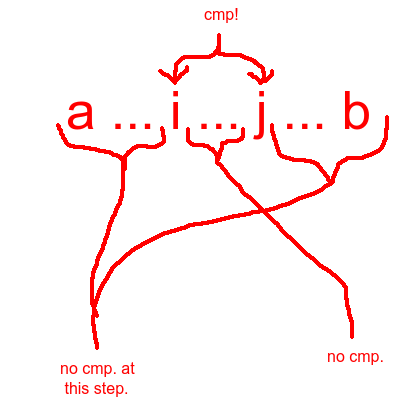
\includegraphics[width=0.6\textwidth]{figures/randqs_lemma.png}
      \caption{Illustration of the three possible cases for $c$.}
      \label{fig:randqs_lemma}
    \end{figure}

    Hence we have:

    \begin{textred}
      \begin{alignat}{3}
                        &X_{ij} &&= [c \in \{i,\ j\} \text{ at some recursive step}],\\
        \text{and}\quad &p_{ij} &&= \frac{2}{j - i + 1},
      \end{alignat}
    \end{textred}

    since the length of the integer interval $\{i,\ \dots,\ j\}$ is $(j - i +
    1)$ and there are two possible ways to achieve what we want.

    So let's substitute the expression for $p_{ij}$ into the summation and start
    working it:

    \begin{textred}
      \begin{align}
         &= \sum_{i = 1}^{n - 1}\sum_{j = i + 1}^n \frac{2}{j - i + 1}\\
         &= \sum_{i = 1}^{n - 1}\sum_{j = 2}^{n - i + 1} \frac{2}{j}\\
         &< \sum_{i = 1}^{n}\sum_{j = 1}^{n} \frac{2}{j}\\
         &= 2n\sum_{j = 1}^{n} \frac{1}{j}\\
         &= 2nH_n\\
         &\leq 2n\ln n\\
         &\in O(n \lg n).
      \end{align}
    \qed
    \end{textred}
\end{enumerate}

\subsubsection{Extras}

\paragraph{Randomized min-cut}

\begin{minted}{text}
RAND_MIN_CUT(V, E):
    V' = {MAKE-SET(v) : v in V}

    C  = empty set
    E' = random permutation of E
    n = |V'|
    for (u, v) in E':
        p_u = find(u)
        p_v = find(v)
        if p_u != p_v:
            if n > 2 then:
                UNION(p_u, p_v)
                n -= 1
            else:
                C += (u, v)
    return C
\end{minted}

\paragraph{Analysis: probabilistic error bound}~\smallskip

Consider some specific \textbf{minimum} cut $C$ with size $k$ of some graph $G =
(V, E)$. For simplicity, assume that $C$ is the only minimum cut of $G$.

Since $C$ has size $k$, we know that each vertex in $G$ must have at least $k$
neighbours, since if there existed a vertex $v$ with less than $k$ neighbors, we
could simply choose a different cut $C'$ which separates $v$ from the rest of
the vertices in $G$.

This lets us put a lower bound on the number of edges in the graph:

\begin{textred}
  \begin{align}
    |E| \geq \frac{nk}{2},
  \end{align}
\end{textred}

where $n = |V|$.

To successfully find the cut $C$, we need to pick edges not in $C$ in every
iteration of the algorithm. In the first iteration, there are $|E|$ edges to
choose from and $k$ edges that we need to avoid, hence the probability of
failure is $1/|E|$ and the probability of success is $1 - k/|E|$:

\begin{textred}
  \begin{align}
    \pr{}{\text{success in first iteration}} &= \frac{k}{|E|}\\
                                             &\leq \frac{k}{nk / 2}\\
                                             &= \frac{2}{n}.
  \end{align}
\end{textred}

In other words, this is the probability of picking an edge that is \emph{not} in
$C$ in a size $n$ graph, and hence we may denote it by $p_{n}$.

\begin{textred}
  \begin{align}
    p_2 &= 1\\
    p_{n} &\geq (1 - 2/n) * p_{n - 1}
  \end{align}
\end{textred}

We expand this to the product:

\begin{textred}
  \begin{align}
    \prod_{i \in \{3, \dots, n\}} \left(1 - \frac{2}{i}\right) \quad&=\quad \prod_{i =
    0}^{n - 3} \left(1 - \frac{2}{n - i}\right)\\
    &=\quad \prod_{i = 0}^{n - 3} \frac{n - i - 2}{n - i}\\
    \quad&=\quad \binom{n}{2}^{-1}\\
         &=\quad \frac{2}{n(n-1)}.
  \end{align}
\end{textred}

In summary, we have:

\begin{textred}
  \begin{align}
    \text{Pr}\left[
      \begin{array}{c}
        \text{respecting a specific } C \text{ throughout}\\
        \text{execution of RAND\_MIN\_CUT}
      \end{array}
      \right]\quad &\geq \quad \quad \binom{n}{2}^{-1}\\
                   &=\quad  \frac{2}{n(n-1)}.
  \end{align}
\end{textred}

If we repeat the algorithm $t$ times, the probability of *\emph{not}* finding a
min cut is:


\begin{textred}
  \begin{align}
    \left(1 - \binom{n}{2}^{-1}\right)^t
  \end{align}
\end{textred}

Choosing $t := \binom{n}{2}\ln n$, we have:

\begin{textred}
  \begin{align}
    \left(1 - \binom{n}{2}^{-1}\right)^{\binom{n}{2} \ln n} \quad\leq \quad\frac{1}{e^{\ln
    n}}\quad =\quad \frac{1}{n}.
  \end{align}
\end{textred}
